\question
$\lim\limits_{x \to 2} \dfrac{x^{2}-4}{x^{2}+4}$ is
\begin{choices}
  \choice $1$
  \CorrectChoice $0$
  \choice $-\dfrac{1}{2}$
  \choice $-1$
  \choice $\infty$
\end{choices}
\begin{solution}
The limit as $x \rightarrow 2$ is $0 \div 8$.
\end{solution}

\question
$\lim\limits_{x \to \infty} \dfrac{4-x^{2}}{x^{2}-1}$ is
\begin{choices}
  \choice $1$
  \choice $0$
  \choice $-4$
  \CorrectChoice $-1$
  \choice $\infty$
\end{choices}
\begin{solution}
Use the Rational Function Theorem (page 96). The degrees of $P(x)$ and $Q(x)$ are the same.
\end{solution}

\question
$\lim\limits_{x \to 3} \dfrac{x-3}{x^{2}-2 x-3}$ is
\begin{choices}
  \choice $0$
  \choice $1$
  \CorrectChoice $\dfrac{1}{4}$
  \choice $\infty$
  \choice none of these
\end{choices}
\begin{solution}
Remove the common factor $x-3$ from numerator and denominator.
\end{solution}

\question
$\lim\limits_{x \to 0} \dfrac{x}{x}$ is
\begin{choices}
  \CorrectChoice $1$
  \choice $0$
  \choice $\infty$
  \choice $-1$
  \choice nonexistent
\end{choices}
\begin{solution}
The fraction equals $1$ for all nonzero $x$.
\end{solution}

\newpage

\question
$\lim\limits_{x \to 2} \dfrac{x^{3}-8}{x^{2}-4}$ is
\begin{choices}
  \choice $4$
  \choice $0$
  \choice $1$
  \CorrectChoice $3$
  \choice $\infty$
\end{choices}
\begin{solution}
Note that $\dfrac{x^{3}-8}{x^{2}-4}=\dfrac{(x-2)\left(x^{2}+2 x+4\right)}{(x-2)(x+2)}$.
\end{solution}

\question
$\lim\limits_{x \to \infty} \dfrac{4-x^{2}}{4 x^{2}-x-2}$ is
\begin{choices}
  \choice $-2$
  \CorrectChoice $-\dfrac{1}{4}$
  \choice $1$
  \choice $2$
  \choice nonexistent
\end{choices}
\begin{solution}
Use the Rational Function Theorem.
\end{solution}

\question
$\lim\limits_{x \to -\infty} \dfrac{5 x^{3}+27}{20 x^{2}+10 x+9}$ is
\begin{choices}
  \CorrectChoice $-\infty$
  \choice $-1$
  \choice $0$
  \choice $3$
  \choice $\infty$
\end{choices}
\begin{solution}
Use the Rational Function Theorem.
\end{solution}

\question
$\lim\limits_{x \to \infty} \dfrac{3 x^{2}+27}{x^{3}-27}$ is
\begin{choices}
  \choice $3$
  \choice $\infty$
  \choice $1$
  \choice $-1$
  \CorrectChoice $0$
\end{choices}
\begin{solution}
Use the Rational Function Theorem.
\end{solution}


\newpage

\question
$\lim\limits_{x \to \infty} \dfrac{2^{-x}}{2^{x}}$ is
\begin{choices}
  \choice $-1$
  \choice $1$
  \CorrectChoice $0$
  \choice $\infty$
  \choice none of these
\end{choices}
\begin{solution}
The fraction is equivalent to $\dfrac{1}{2^{2 x}}$; the denominator approaches $\infty$.
\end{solution}

\question
$\lim\limits_{x \to -\infty} \dfrac{2^{-x}}{2^{x}}$ is
\begin{choices}
  \choice $-1$
  \choice $1$
  \choice $0$
  \CorrectChoice $\infty$
  \choice none of these
\end{choices}
\begin{solution}
Since $\dfrac{2^{-x}}{2^{x}}=2^{-2 x}$, therefore, as $x \rightarrow-\infty$, the fraction $\rightarrow+\infty$.
\end{solution}

\question
$\lim\limits_{x \to 0} \dfrac{\sin 5 x}{x}$
\begin{choices}
  \choice $=0$
  \choice $=\dfrac{1}{5}$
  \choice $=1$
  \CorrectChoice $=5$
  \choice does not exist
\end{choices}
\begin{solution}
$\lim\limits_{x \to 0} \dfrac{\sin 5 x}{x}=\lim\limits_{x \to 0} \dfrac{\sin 5 x}{x} \cdot \dfrac{5}{5}=5 \lim\limits_{x \to 0} \dfrac{\sin 5 x}{5 x}=5$.
\end{solution}


\newpage

\question
$\lim\limits_{x \to 0} \dfrac{\sin 2 x}{3 x}$
\begin{choices}
  \choice $=0$
  \CorrectChoice $=\dfrac{2}{3}$
  \choice $=1$
  \choice $=\dfrac{3}{2}$
  \choice does not exist
\end{choices}
\begin{solution}
$\lim\limits_{x \to 0} \dfrac{\sin 2 x}{3 x}=\dfrac{1}{3} \lim\limits_{x \to 0} \dfrac{\sin 2 x}{x} \cdot \dfrac{2}{2}=\dfrac{2}{3} \lim\limits_{x \to 0} \dfrac{\sin 2 x}{2 x}=\dfrac{2}{3}$.
\end{solution}

\question
The graph of $y=\arctan x$ has
\begin{choices}
  \choice vertical asymptotes at $x=0$ and $x=\pi$
  \CorrectChoice horizontal asymptotes at $y=\pm \dfrac{\pi}{2}$
  \choice horizontal asymptotes at $y=0$ and $y=\pi$
  \choice vertical asymptotes at $x=\pm \dfrac{\pi}{2}$
  \choice none of these
\end{choices}
\begin{solution}
Because the graph of $y=\tan x$ has vertical asymptotes at $x=\pm \dfrac{\pi}{2}$, the graph of the inverse function $y=\arctan x$ has horizontal asymptotes at $y=\pm \dfrac{\pi}{2}$.
\end{solution}

\question
The graph of $y=\dfrac{x^{2}-9}{3 x-9}$ has
\begin{choices}
  \choice a vertical asymptote at $x=3$
  \choice a horizontal asymptote at $y=\dfrac{1}{3}$
  \CorrectChoice a removable discontinuity at $x=3$
  \choice an infinite discontinuity at $x=3$
  \choice none of these
\end{choices}
\begin{solution}
Since $\dfrac{x^{2}-9}{3 x-9}=\dfrac{(x-3)(x+3)}{3(x-3)}=\dfrac{x+3}{3}$ (provided $x \neq 3$), $y$ can be defined to be equal to $2$ at $x=3$, removing the discontinuity at that point.
\end{solution}


\newpage

\question
$\lim\limits_{x \to 0} \dfrac{\sin x}{x^{2}+3 x}$ is
\begin{choices}
  \choice $1$
  \CorrectChoice $\dfrac{1}{3}$
  \choice $3$
  \choice $\infty$
  \choice $\dfrac{1}{4}$
\end{choices}
\begin{solution}
Note that $\dfrac{\sin x}{x^{2}+3 x}=\dfrac{\sin x}{x(x+3)}=\dfrac{\sin x}{x} \cdot \dfrac{1}{x+3} \rightarrow 1 \cdot \dfrac{1}{3}$.
\end{solution}

\question
$\lim\limits_{x \to 0} \sin \dfrac{1}{x}$ is
\begin{choices}
  \choice $\infty$
  \choice $1$
  \CorrectChoice nonexistent
  \choice $-1$
  \choice none of these
\end{choices}
\begin{solution}
As $x \rightarrow 0$, $\dfrac{1}{x}$ takes on varying finite values as it increases. Since the sine function repeats, $\sin \dfrac{1}{x}$ oscillates, taking on, infinitely many times, each value between $-1$ and $1$. The calculator graph of $Y_{1}=\sin (1/X)$ exhibits this oscillating discontinuity at $x=0$.
\end{solution}

\question
Which statement is true about the curve $y=\dfrac{2 x^{2}+4}{2+7 x-4 x^{2}}$?
\begin{choices}
  \CorrectChoice The line $x=-\dfrac{1}{4}$ is a vertical asymptote.
  \choice The line $x=1$ is a vertical asymptote.
  \choice The line $y=-\dfrac{1}{4}$ is a horizontal asymptote.
  \choice The graph has no vertical or horizontal asymptote.
  \choice The line $y=2$ is a horizontal asymptote.
\end{choices}
\begin{solution}
Note that, since $y=\dfrac{2 x^{2}+4}{(2-x)(1+4 x)}$, both $x=2$ and $x=-\dfrac{1}{4}$ are vertical asymptotes. Also, $y=-\dfrac{1}{2}$ is a horizontal asymptote.
\end{solution}

\newpage


\question
$\lim\limits_{x \to \infty} \dfrac{2 x^{2}+1}{(2-x)(2+x)}$ is
\begin{choices}
  \choice $-4$
  \CorrectChoice $-2$
  \choice $1$
  \choice $2$
  \choice nonexistent
\end{choices}
\begin{solution}
$\dfrac{2 x^{2}+1}{(2-x)(2+x)}=\dfrac{2 x^{2}+1}{4-x^{2}}$. Use the Rational Function Theorem (page 96).
\end{solution}

\question
$\lim\limits_{x \to 0} \dfrac{|x|}{x}$ is
\begin{choices}
  \choice $0$
  \CorrectChoice nonexistent
  \choice $1$
  \choice $-1$
  \choice none of these
\end{choices}
\begin{solution}
Since $|x|=x$ if $x>0$ but equals $-x$ if $x<0$, $\lim\limits_{x \to 0^{+}} \dfrac{|x|}{x}=\lim\limits_{x \to 0^{+}} \dfrac{x}{x}=1$ while $\lim\limits_{x \to 0^{-}} \dfrac{|x|}{x}=\lim\limits_{x \to 0^{-}} \dfrac{-x}{x}=-1$.
\end{solution}

\question
$\lim\limits_{x \to \infty} x \sin \dfrac{1}{x}$ is
\begin{choices}
  \choice $0$
  \choice $\infty$
  \choice nonexistent
  \choice $-1$
  \CorrectChoice $1$
\end{choices}
\begin{solution}
Note that $x \sin \dfrac{1}{x}$ can be rewritten as $\dfrac{\sin \dfrac{1}{x}}{\dfrac{1}{x}}$ and that, as $x \rightarrow \infty$, $\dfrac{1}{x} \rightarrow 0$.
\end{solution}


\newpage

\question
$\lim\limits_{x \to \pi} \dfrac{\sin (\pi-x)}{\pi-x}$ is
\begin{choices}
  \CorrectChoice $1$
  \choice $0$
  \choice $\infty$
  \choice nonexistent
  \choice none of these
\end{choices}
\begin{solution}
As $x \rightarrow \pi$, $(\pi-x) \rightarrow 0$.
\end{solution}

\question
Let
\[
f(x)= \begin{cases}\dfrac{x^{2}-1}{x-1} & \text{if } x \neq 1 \\ 4 & \text{if } x=1.\end{cases}
\]
Which of the following statements is (are) true?
\statementbox{%
\begin{enumerate}
\renewcommand{\labelenumi}{\Roman{enumi}.}
  \item $\lim\limits_{x \to 1} f(x)$ exists
  \item $f(1)$ exists
  \item $f$ is continuous at $x=1$
\end{enumerate}%
}
\begin{choices}
  \choice I only
  \choice II only
  \CorrectChoice I and II
  \choice none of them
  \choice all of them
\end{choices}
\begin{solution}
Since $f(x)=x+1$ if $x \neq 1$, $\lim\limits_{x \to 1} f(x)$ exists (and is equal to $2$).
\end{solution}

\question
If
\[
f(x)=\begin{cases}\dfrac{x^{2}-x}{2 x} & \text{for } x \neq 0 \\ k & \text{at } x=0,\end{cases}
\]
and if $f$ is continuous at $x=0$, then $k=$
\begin{choices}
  \choice $-1$
  \CorrectChoice $-\dfrac{1}{2}$
  \choice $0$
  \choice $\dfrac{1}{2}$
  \choice $1$
\end{choices}
\begin{solution}
$f(x)=\dfrac{x(x-1)}{2 x}=\dfrac{x-1}{2}$, for all $x \neq 0$. For $f$ to be continuous at $x=0$, $\lim\limits_{x \to 0} f(x)$ must equal $f(0)$. $\lim\limits_{x \to 0} f(x)=-\dfrac{1}{2}$.
\end{solution}


\newpage

\question
Suppose
\[
f(x)=\begin{cases}\dfrac{3 x(x-1)}{x^{2}-3 x+2} & \text{for } x \neq 1,2 \\ -3 & \text{at } x=1 \\ 4 & \text{at } x=2.\end{cases}
\]
Then $f(x)$ is continuous
\begin{choices}
  \choice except at $x=1$
  \CorrectChoice except at $x=2$
  \choice except at $x=1$ or $2$
  \choice except at $x=0$, $1$, or $2$
  \choice at each real number
\end{choices}
\begin{solution}
Only $x=1$ and $x=2$ need be checked. Since $f(x)=\dfrac{3 x}{x-2}$ for $x \neq 1,2$, and $\lim\limits_{x \to 1} f(x)=-3=f(1)$, $f$ is continuous at $x=1$. Since $\lim\limits_{x \to 2} f(x)$ does not exist, $f$ is not continuous at $x=2$.
\end{solution}

\question
The graph of $f(x)=\dfrac{4}{x^{2}-1}$ has
\begin{choices}
  \choice one vertical asymptote, at $x=1$
  \choice the $y$-axis as vertical asymptote
  \CorrectChoice the $x$-axis as horizontal asymptote and $x=\pm 1$ as vertical asymptotes
  \choice two vertical asymptotes, at $x=\pm 1$, but no horizontal asymptote
  \choice no asymptote
\end{choices}
\begin{solution}
As $x \rightarrow \pm \infty$, $y=f(x) \rightarrow 0$, so the $x$-axis is a horizontal asymptote. Also, as $x \rightarrow \pm 1$, $y \rightarrow \infty$, so $x=\pm 1$ are vertical asymptotes.
\end{solution}

\question
The graph of $y=\dfrac{2 x^{2}+2 x+3}{4 x^{2}-4 x}$ has
\begin{choices}
  \choice a horizontal asymptote at $y=+\dfrac{1}{2}$ but no vertical asymptote
  \choice no horizontal asymptote but two vertical asymptotes, at $x=0$ and $x=1$
  \CorrectChoice a horizontal asymptote at $y=\dfrac{1}{2}$ and two vertical asymptotes, at $x=0$ and $x=1$
  \choice a horizontal asymptote at $x=2$ but no vertical asymptote
  \choice a horizontal asymptote at $y=\dfrac{1}{2}$ and two vertical asymptotes, at $x=\pm 1$
\end{choices}
\begin{solution}
As $x \rightarrow \infty$, $y \rightarrow \dfrac{1}{2}$; the denominator (but not the numerator) of $y$ equals $0$ at $x=0$ and at $x=1$.
\end{solution}


\newpage

\question
Let
\[
f(x)=\begin{cases}\dfrac{x^{2}+x}{x} & \text{if } x \neq 0 \\ 1 & \text{if } x=0.\end{cases}
\]
Which of the following statements is (are) true?
\statementbox{%
\begin{enumerate}
\renewcommand{\labelenumi}{\Roman{enumi}.}
  \item $f(0)$ exists
  \item $\lim\limits_{x \to 0} f(x)$ exists
  \item $f$ is continuous at $x=0$
\end{enumerate}%
}
\begin{choices}
  \choice I only
  \choice II only
  \choice I and II only
  \CorrectChoice all of them
  \choice none of them
\end{choices}
\begin{solution}
The function is defined at $0$ to be $1$, which is also $\lim\limits_{x \to 0} \dfrac{x^{2}+x}{x}=\lim\limits_{x \to 0}(x+1)$.
\end{solution}

\question\label{calc02:floor-half}
If $[x]$ is the greatest integer not greater than $x$, then $\lim\limits_{x \to 1/2}[x]$ is
\begin{choices}
  \choice $\dfrac{1}{2}$
  \choice $1$
  \choice nonexistent
  \CorrectChoice $0$
  \choice none of these
\end{choices}
\begin{solution}
See Figure N2-1 on page 88.
\end{solution}

\question
(With the same notation as in Question~\ref{calc02:floor-half}) $\lim\limits_{x \to -2}[x]$ is
\begin{choices}
  \choice $-3$
  \choice $-2$
  \choice $-1$
  \choice $0$
  \CorrectChoice none of these
\end{choices}
\begin{solution}
Note, from Figure N2-1, that $\lim\limits_{x \to -2^{-}}[x]=-3$ but $\lim\limits_{x \to -2^{+}}[x]=-2$.
\end{solution}


\newpage

\question
$\lim\limits_{x \to \infty} \sin x$
\begin{choices}
  \choice is $-1$
  \choice is infinity
  \choice oscillates between $-1$ and $1$
  \choice is zero
  \CorrectChoice does not exist
\end{choices}
\begin{solution}
As $x \rightarrow \infty$, the function $\sin x$ oscillates between $-1$ and $1$; hence the limit does not exist.
\end{solution}

\question
The function
\[
f(x)= \begin{cases}x^{2}/x & (x \neq 0) \\ 0 & (x=0)\end{cases}
\]
\begin{choices}
  \CorrectChoice is continuous everywhere
  \choice is continuous except at $x=0$
  \choice has a removable discontinuity at $x=0$
  \choice has an infinite discontinuity at $x=0$
  \choice has $x=0$ as a vertical asymptote
\end{choices}
\begin{solution}
Note that $\dfrac{x^{2}}{x}=x$ if $x \neq 0$ and that $\lim\limits_{x \to 0} f=0$.
\end{solution}

\newpage

\begin{EnvFullwidth}
\textit{Questions~\ref{calc02:piecewise-first}--\ref{calc02:piecewise-last} are based on the function $f$ shown in the graph and defined below.}

\begin{multicols}{2}
\noindent
$\displaystyle
f(x)=\begin{cases}
1-x & (-1 \leqq x<0) \\
2 x^{2}-2 & (0 \leqq x \leqq 1) \\
-x+2 & (1<x<2) \\
1 & (x=2) \\
2 x-4 & (2<x \leqq 3)
\end{cases}$
\columnbreak
\centering
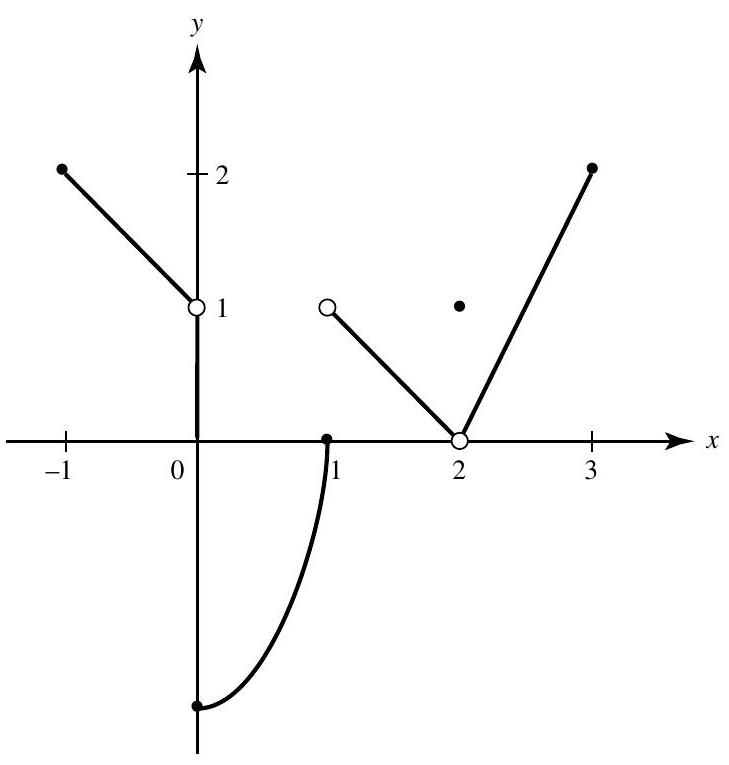
\includegraphics[width=\linewidth]{calculus/images/c695ae97-6a0d-4fa2-869d-3f974eff86fb-5_765_729_296_1308.jpg}
\end{multicols}
\end{EnvFullwidth}

\question\label{calc02:piecewise-first}
$\lim\limits_{x \to 2} f(x)$
\begin{choices}
  \CorrectChoice equals $0$
  \choice equals $1$
  \choice equals $2$
  \choice does not exist
  \choice none of these
\end{choices}
\begin{solution}
$\lim\limits_{x \to 2^{-}} f(x)=\lim\limits_{x \to 2^{+}} f(x)=0$.
\end{solution}

\question
The function $f$ is defined on $[-1,3]$
\begin{choices}
  \choice if $x \neq 0$
  \choice if $x \neq 1$
  \choice if $x \neq 2$
  \choice if $x \neq 3$
  \CorrectChoice at each $x$ in $[-1,3]$
\end{choices}
\begin{solution}
Verify that $f$ is defined at $x=0$, $1$, $2$, and $3$ (as well as at all other points in $[-1,3]$).
\end{solution}



\newpage



\question
The function $f$ has a removable discontinuity at
\begin{choices}
  \choice $x=0$
  \choice $x=1$
  \CorrectChoice $x=2$
  \choice $x=3$
  \choice none of these
\end{choices}
\begin{solution}
Note that $\lim\limits_{x \to 2^{-}} f(x)=\lim\limits_{x \to 2^{+}} f(x)=0$. However, $f(2)=1$. Redefining $f(2)$ as $0$ removes the discontinuity.
\end{solution}

\question
On which of the following intervals is $f$ continuous?
\begin{choices}
  \choice $-1 \leqq x \leqq 0$
  \CorrectChoice $0<x<1$
  \choice $1 \leqq x \leqq 2$
  \choice $2 \leqq x \leqq 3$
  \choice none of these
\end{choices}
\begin{solution}
The function is not continuous at $x=0$, $1$, or $2$.
\end{solution}

\question\label{calc02:piecewise-last}
The function $f$ has a jump discontinuity at
\begin{choices}
  \choice $x=-1$
  \CorrectChoice $x=1$
  \choice $x=2$
  \choice $x=3$
  \choice none of these
\end{choices}
\begin{solution}
$\lim\limits_{x \to 1^{-}} f(x)=0 \neq \lim\limits_{x \to 1^{+}} f(x)=1$.
\end{solution}




\newpage



\question
Suppose $\lim\limits_{x \to -3^{-}} f(x)=-1$, $\lim\limits_{x \to -3^{+}} f(x)=-1$, and $f(-3)$ is not defined. Which of the following statements is (are) true?
\statementbox{%
\begin{enumerate}
\renewcommand{\labelenumi}{\Roman{enumi}.}
  \item $\lim\limits_{x \to -3} f(x)=-1$.
  \item $f$ is continuous everywhere except at $x=-3$.
  \item $f$ has a removable discontinuity at $x=-3$.
\end{enumerate}%
}
\begin{choices}
  \choice None of them
  \choice I only
  \choice III only
  \CorrectChoice I and III only
  \choice All of them
\end{choices}
\begin{solution}
No information is given about the domain of $f$ except in the neighborhood of $x=-3$.
\end{solution}

\question
If $y=\dfrac{1}{2+10^{\dfrac{1}{x}}}$, then $\lim\limits_{x \to 0} y$ is
\begin{choices}
  \choice $0$
  \choice $\dfrac{1}{12}$
  \choice $\dfrac{1}{2}$
  \choice $\dfrac{1}{3}$
  \CorrectChoice nonexistent
\end{choices}
\begin{solution}
As $x \rightarrow 0^{+}$, $10^{\dfrac{1}{x}} \rightarrow \infty$ and therefore $y \rightarrow 0$. As $x \rightarrow 0^{-}$, $\dfrac{1}{x} \rightarrow-\infty$, so $10^{\dfrac{1}{x}} \rightarrow 0$ and therefore $y \rightarrow \dfrac{1}{2}$. Because the two one-sided limits are not equal, the limit does not exist. (Verify with a calculator.)
\end{solution}

\question
$\lim\limits_{x \to 0} \sqrt{3+\arctan \dfrac{1}{x}}$ is
\begin{choices}
  \choice $-\infty$
  \choice $\sqrt{3-\dfrac{\pi}{2}}$
  \choice $\sqrt{3+\dfrac{\pi}{2}}$
  \choice $\infty$
  \CorrectChoice none of these
\end{choices}
\begin{solution}
As $x \rightarrow 0^{-}$, $\arctan \dfrac{1}{x} \rightarrow-\dfrac{\pi}{2}$, so $y \rightarrow \sqrt{3-\dfrac{\pi}{2}}$. As $x \rightarrow 0^{+}$, $y \rightarrow \sqrt{3+\dfrac{\pi}{2}}$. The graph has a jump discontinuity at $x=0$. (Verify with a calculator.)

\medskip
\noindent\textit{*Challenge question: may be more difficult than typical AP Calculus exam items.}
\end{solution}
